\documentclass[12pt]{article}
\usepackage{fancyhdr}
\usepackage{amsmath,amsthm,amssymb,dsfont,enumerate,color}
\usepackage[top=1in, bottom=1in]{geometry}
\usepackage{tikz}
\usepackage{tikz-3dplot}
\usetikzlibrary{patterns}
\tdplotsetmaincoords{70}{110}
\usetikzlibrary{arrows.meta}
\fancyhead[L]{MAT473}
\fancyhead[R]{Homework 3}
\fancyfoot[L]{Name: \underline{\hspace{2in}}}
\fancyfoot[R]{\large \thepage}
\fancyfoot[C]{}
\newcommand{\bbA}{\mathbb{A}}
\newcommand{\bbB}{\mathbb{B}}
\newcommand{\bbC}{\mathbb{C}}
\newcommand{\bbD}{\mathbb{D}}
\newcommand{\bbE}{\mathbb{E}}
\newcommand{\bbF}{\mathbb{F}}
\newcommand{\bbG}{\mathbb{G}}
\newcommand{\bbH}{\mathbb{H}}
\newcommand{\bbI}{\mathbb{I}}
\newcommand{\bbJ}{\mathbb{J}}
\newcommand{\bbK}{\mathbb{K}}
\newcommand{\bbL}{\mathbb{L}}
\newcommand{\bbM}{\mathbb{M}}
\newcommand{\bbN}{\mathbb{N}}
\newcommand{\bbO}{\mathbb{O}}
\newcommand{\bbP}{\mathbb{P}}
\newcommand{\bbQ}{\mathbb{Q}}
\newcommand{\bbR}{\mathbb{R}}
\newcommand{\R}{\mathbb{R}}
\newcommand{\bbS}{\mathbb{S}}
\newcommand{\bbT}{\mathbb{T}}
\newcommand{\bbU}{\mathbb{U}}
\newcommand{\bbV}{\mathbb{V}}
\newcommand{\bbW}{\mathbb{W}}
\newcommand{\bbX}{\mathbb{X}}
\newcommand{\bbY}{\mathbb{Y}}
\newcommand{\bbZ}{\mathbb{Z}}
\newcommand{\bbk}{\mathbb{k}}

\newcommand{\calA}{\mathcal{A}}
\newcommand{\calB}{\mathcal{B}}
\newcommand{\calC}{\mathcal{C}}
\newcommand{\calD}{\mathcal{D}}
\newcommand{\calE}{\mathcal{E}}
\newcommand{\calF}{\mathcal{F}}
\newcommand{\calG}{\mathcal{G}}
\newcommand{\calH}{\mathcal{H}}
\newcommand{\calI}{\mathcal{I}}
\newcommand{\calJ}{\mathcal{J}}
\newcommand{\calK}{\mathcal{K}}
\newcommand{\calL}{\mathcal{L}}
\newcommand{\calM}{\mathcal{M}}
\newcommand{\calN}{\mathcal{N}}
\newcommand{\calO}{\mathcal{O}}
\newcommand{\calP}{\mathcal{P}}
\newcommand{\calQ}{\mathcal{Q}}
\newcommand{\calR}{\mathcal{R}}
\newcommand{\calS}{\mathcal{S}}
\newcommand{\calT}{\mathcal{T}}
\newcommand{\calU}{\mathcal{U}}
\newcommand{\calV}{\mathcal{V}}
\newcommand{\calW}{\mathcal{W}}
\newcommand{\calX}{\mathcal{X}}
\newcommand{\calY}{\mathcal{Y}}
\newcommand{\calZ}{\mathcal{Z}}
\newcommand{\iitem}{\vfill \item}
\newcommand{\topic}[1]{\textcolor{blue}{#1}}
\newcommand{\answerbox}{\begin{flushright}
    \begin{tikzpicture}
      \draw (0,0) rectangle (5,-1.75);
    \end{tikzpicture}\end{flushright}}
\newcommand{\solution}[1]{\textcolor{red}{#1}}
\newcommand{\points}[1]{\ [#1pts]}
%\renewcommand{\solution}[1]{}

\begin{document}
\pagestyle{fancy}

Throughout we assume that $R$ is a commutative ring with identity
$1\neq 0$.
\begin{enumerate}
\item Recall that $S^{-1}R$ is defined to be the set of equivalence
  classes in $R\times S$ with the equivalence relation $(r,s)\sim
  (r',s')$ if there exists an element $t\in S$ such that
  $t(rs'-r's)=0$. Prove that the multiplication $(r_1,s_1)\cdot
  (r_2,s_2)=(r_1r_2,s_1s_2)$ is a well-defined operation on
  $S^{-1}R$. 
\solution{
Let $(r,s)\sim (r',s')$ and choose $t$ so that $t(rs'-r's)=0$. Then we
compute:
\begin{align*}
  (r,s)(a,b) &= (ra,sb)\\
(r',s')(a,b) &= (r'a,s'b).
\end{align*}
I claim that $(r'a,s'b)\sim (ra,sb)$. Indeed, $t(r'asb-ras'b) =
t(r's-rs')ab = 0 \cdot ab = 0$. So multiplication is well-defined on
$S^{-1}R$. 
}
\item Define $\Phi$ to be the
  function which takes a subset of $R$ to a subset of $S^{-1}R$ in the
  following way: 
  \[\Phi(I) = \{(x,s) \mid x\in I, s\in S\}.\]
  \begin{itemize}
  \item Prove that if $I$ is an ideal in $R$, then $\Phi(I)$ is an
    ideal in $S^{-1}R$. 
\solution{Suppose that $I$ is an ideal in $R$. Let $(x,s), (y,s')\in \Phi(I)$ and
  $(r,s'') \in S^{-1}R$. By definition, $x,y\in I$. Then
  $(x,s)+(r,s'')(y,s') = (xs'+sry,ss's'')$ is in $\Phi(I)$ since
  $xs'\in I$ and $sry\in I$. Also $(0,1)\in \Phi(I)$ since $0\in I$. }
  \item Prove that if $P$ is a prime ideal that does not intersect
    $S$, and $S$ has no zero divisors, then $\Phi(I)$ is a prime ideal
    in $S^{-1}R$. 
\solution{Suppose that $P$ is a prime ideal not intersecting $S$ and
  that $S$ has no zero divisors. Suppose that $(x,s)(y,s')\in
  \Phi(I).$ Then $(xy,ss')\in \Phi(I)$, i.e., there is an element
  $r\in I$ such that $(xy,ss')\sim (r,s'')$ for some $s''$. This
  implies there exists a $t\in S$ such that $t(xys''-rss')=0$. Since
  $S$ has no zero-divisors, $xys''=rss'\in I$ since $r\in I$. Since
  $s''\notin I$, this implies $xy\in I$, so either $x\in I$ or $y\in
  I$.} 
  \end{itemize}


\item Suppose that $S\subset R$ is a multiplicative set in $R$. Prove
  that the homomorphism $\phi: R\rightarrow S^{-1}R$ is injective if
  and only if $S$ contains no zero-divisors. 
\solution{
Suppose that $\phi$ is injective and that $s \in S$ such that $rs=0$
for some $r\in R$.
\begin{align*}
 (0,1) &= \phi(0)\\ &= \phi(rs) \\ &= (rs,1).
\end{align*}
Since $s\in S$, there is an element $(1,s)$ in $S^{-1}R$ with the
property that $(1,s)(s,1)=(s,s)=(1,1)$ (the latter equality due to the
fact that $t(s-s)=0$ for any $t$ we choose). Multiplying both sides of
the equation by this element yields
\begin{align*}
  (0,1)(1,s) &= (r,1)(s,1)(1,2)\\
(0,s) &= (r,1). 
\end{align*}
Hence, $\phi(r)=0$, which implies $r=0$. Thus, $s$ is not a
zero-divisor.
Next, suppose that $S$ has a zero divisor $t$ such that $tr=0$ for
some non-zero $r\in R$. Then I claim that $(r,1)=(0,1)$ in
$S^{-1}R$. Indeed, $t(r\cdot 1 - 0 \cdot 1) = tr = 0$. So
$\phi(r)=(r,1)=0$. Hence, $\phi$ is not injective. 
}
\item Let $p$ be a prime integer, and consider the ring $R=\bbZ$. Let
  $S=\bbZ \setminus p\bbZ$. The ring $S^{-1}R$ is called the
  localization of $\bbZ$ at $p$. Find all of the ideals of this ring,
  and describe the maximal ideal (there is only one).
\solution{We proved in class that $\Phi$ from problem 2 is a bijection
  between ideals in $R$ not intersecting $S$ and ideals in
  $S^{-1}R$. Let $n\bbZ$ be an ideal in $\bbZ$ such that $n\bbZ \cap
  S=\emptyset$. Then
  \begin{align*}
    n\bbZ \cap (\bbZ\setminus p\bbZ) &= \emptyset \\
\Rightarrow n\bbZ \setminus n\bbZ \cap p\bbZ &= \emptyset\\
\Rightarrow n\bbZ \setminus np \bbZ &= \emptyset\\
\Rightarrow n=kp & \exists k\in \bbZ.
  \end{align*}
So the ideals in $S^{-1}R$ are the ideals generated by a multiple of
$p$. These are all contained in $p\bbZ$, so this is the unique maximal
ideal. }

\item This problem is to help us look ahead. Let $\varphi(n)$ denote
  the number of units in $\bbZ/n\bbZ$. (From previous homework, we
  know this is the same as computing the number of integers $1\leq k<n$
  that are relatively prime to $n$.)
\begin{enumerate}
\item Compute $\varphi(p^k)$ when $p$ is prime and $k$ is a
  non-negative integer.
\solution{Write the element $m\in \bbZ/p^k \bbZ$ as
  $\sum\limits_{i=0}^{k-1} a_i p^i$ where $a_i \in \{0,\dotsc,
  p-1\}$. Then $m$ is a unit if and only if $a_0\neq 0$. This yields
  $(p-1)p^{k-1}$ elements.}
\item Compute $\varphi(n)$ for $n\in \{6, 10, 12, 18, 24, 36\}$ and make a
  conjecture about the relationship between $\varphi(n)$ and the prime
  power decomposition of $n$. \solution{Good guess: $\varphi(n) =
    \prod_i \varphi(p_i^{k_i})$ when $n=\prod_i p_i^{k_i}$.}
\end{enumerate}

\end{enumerate}
Here I'll recall the universal property that defines a product, and
introduce a new one that defines the coproduct. 

\fbox{\begin{minipage}{0.95\linewidth}
{\bf Definition:} Let $X_1, X_2$ be objects in a category $\calC$. Define $X_1 \prod X_2$
  to be the object with the following universal property: There are
  morphisms $\pi_i: X_1\prod X_2 \rightarrow X_i$ such that if there
  is any other object $T$ with morphisms $\varphi_i: T\rightarrow X_i$
  for $i\in \{1,2\}$, then there is a unique morphism $\Psi:
  T\rightarrow X_1 \times\prod X_2$ such that $\pi_i \circ \Psi =
  \varphi_i$. 
\end{minipage}}

\begin{minipage}{0.55\linewidth}This is conveniently captured in the diagram to the right, and is read to mean that you start with the
  object $X_1 \prod X_2$ and its morphisms to $X_1$ and $X_2$ set in
  stone. Any time there is an object $T$ with morphisms as in the
  diagram, there is a morphism $\Psi$ that can fill in that dotted
  arrow so that the diagram commutes, meaning any two ways to get to
  the same place produce the same morphism. 
\end{minipage} \begin{minipage}{0.4\linewidth}
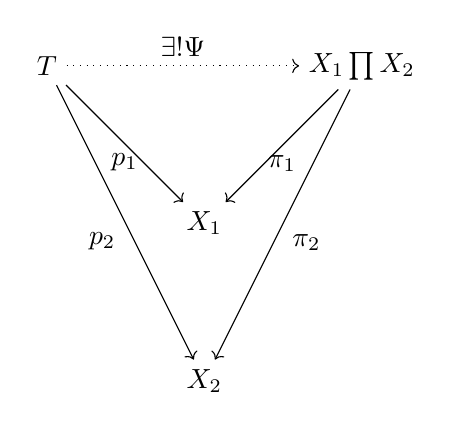
\begin{tikzpicture}
    \node (T) at (-2,0) {$T$};
    \node (prod) at (2,0) {$X_1 \prod X_2$};
    \node (X1) at (0,-2) {$X_1$};
    \node (X2) at (0,-4) {$X_2$};
    \draw[->] (T)--(X1) node[midway, below] {$p_1$};
    \draw[->] (T)--(X2) node[midway, below left] {$p_2$};
    \draw[->] (prod)--(X1) node[midway, below] {$\pi_1$};
    \draw[->] (prod)--(X2) node[midway, below right] {$\pi_2$};
    \draw[dotted,->] (T)--(prod) node[midway, above] {$\exists ! \Psi$};
  \end{tikzpicture}\end{minipage}
\begin{enumerate}
\item[6.] Prove that if $R_1$ and $R_2$ are rings, then the
  product ring $\{(r_1,r_2) \mid r_1\in R_1, r_2\in R_2\}$ is actually
  the object $R_1 \prod R_2$. I.e., verify that it satisfies the
  universal property. 
\solution{
Clearly we have maps $f_i: R_1 \times R_2 \rightarrow R_i$ given by
$f_i(r_1,r_2)=r_i$. Now suppose that $T$ is a ring with homomorphisms
$p_i: T\rightarrow R_i$. Then define $\Phi: T\rightarrow R_1\times
R_2$ via $\Phi(t) = (p_1(t), p_2(t))$. We verify:
$\pi_i(\Phi(t))=p_i(t)$, so the diagram commutes. Furthermore, if
$f(t)=(f_1(t),f_2(t))$, then $\pi_i(f(t))=f_i(t)$, so in order for the
commutativity to hold, $f_i(t)=p_i(t)$. Hence, $\Phi=f$, so $\Phi$ is
the unique morphism making the commutativity hold.}
\item[7.] Consider now the category $\calC$ whose objects are positive
  integers and so that $\operatorname{Mor}_\calC(n,m) =\begin{cases}
    \{m/n\} & \textrm{ if } n\mid m\\
\emptyset & \textrm{ otherwise}\end{cases}.$ Given two integers $n,m$,
compute $m \prod n$ in this context (i.e., what integer has the
desired universal property). 
\end{enumerate}
If you really like the last problem, awesome. You can try your hand at
a new one. This is just for the superfans. Try to write what you think
the universal property of the coproduct should be given just the
diagram: 

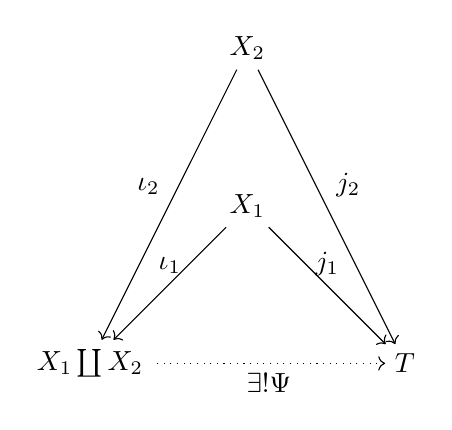
\begin{tikzpicture}
      \node (T) at (2,0) {$T$};
    \node (prod) at (-2,0) {$X_1 \coprod X_2$};
    \node (X1) at (0,2) {$X_1$};
    \node (X2) at (0,4) {$X_2$};
    \draw[<-] (T)--(X1) node[midway, above] {$j_1$};
    \draw[<-] (T)--(X2) node[midway, above right] {$j_2$};
    \draw[<-] (prod)--(X1) node[midway, above] {$\iota_1$};
    \draw[<-] (prod)--(X2) node[midway, above left] {$\iota_2$};
    \draw[dotted,<-] (T)--(prod) node[midway, below] {$\exists ! \Psi$};
\end{tikzpicture}

Then, compute $m\coprod n$ for objects $m,n$ in $\calC$. 
\solution{Suppose that $m,n\in \bbZ_{>0}$. I claim that $m\prod n =
  \gcd(m,n).$ First, since $\gcd(m,n)\mid m$ and $\gcd(m,n)\mid n$, we
  have morphisms $\pi_m: \gcd(m,n) \rightarrow m$ and $\pi_n:
  \gcd(m,n)\rightarrow n$ (encoded as $m/\gcd(m,n)$ and $n/\gcd(m,n)$). Now suppose that there is an integer $t$
  and morphisms $p_m: t\rightarrow m$ and $p_n: t\rightarrow n$. By
  definition, then, $t\mid m$ and $t\mid n$  (and they are encoded as $m/t$ and $n/t$). If this is the case, then
  $t\mid \gcd(m,n)$, so there is a morphism $\Phi: t\rightarrow
  \gcd(m,n)$ (encoded as $\gcd(m,n)/t$). Note that $\pi_m \circ \Phi$
  is encoded as $(m/\gcd(m,n))(\gcd(m,n)/t)=m/t$ and similarly for
  $n$. Thus, $\pi_\star \Phi= p_\star$, and since the morphism sets
  here are singletons, $\Phi$ is unique.}
\end{document}
2018/01/17 18:53:34
